\documentclass[11pt]{article}

% Packages
\usepackage[margin=1in]{geometry}
\usepackage{amsmath,amssymb,amsthm,mathtools}
\usepackage{hyperref}
\usepackage{booktabs}
\usepackage{graphicx}
\usepackage{natbib}
\usepackage{tikz}
\usetikzlibrary{fit,backgrounds,bayesnet}
\usepackage{caption}
\usepackage{multirow}
\usepackage{array}

% Hyperref setup
\hypersetup{
    colorlinks=true,
    linkcolor=blue,
    citecolor=blue,
    urlcolor=blue
}

% Theorem environments
\theoremstyle{definition}
\newtheorem{condition}{Condition}
\newtheorem{definition}{Definition}
\newtheorem{example}{Example}
\newtheorem{remark}{Remark}

\theoremstyle{plain}
\newtheorem{theorem}{Theorem}
\newtheorem{lemma}{Lemma}
\newtheorem{proposition}{Proposition}
\newtheorem{corollary}{Corollary}

% Custom commands
\renewcommand{\v}[1]{\boldsymbol{#1}}
\newcommand{\btheta}{\v{\theta}}
\newcommand{\bomega}{\v{\Omega}}
\newcommand{\E}{\mathbb{E}}

\title{Masked Causes of Failure in Series Systems:\\
A Likelihood Framework}

\author{
    Alexander Towell\\
    \href{mailto:lex@metafunctor.com}{lex@metafunctor.com}\\
    \href{https://orcid.org/0000-0001-6443-9897}{ORCID: 0000-0001-6443-9897}
}

\date{February 2026}

\begin{document}

\maketitle

\begin{abstract}
We develop a general likelihood framework for estimating component reliability
from series system data when the component cause of failure is masked.
The framework applies to any parametric specification of component hazard
functions, including covariate-dependent hazards.
Three sufficient conditions on the masking mechanism---that the candidate set
contains the true cause, that masking probabilities are symmetric across
candidates, and that masking probabilities are independent of the component
lifetime parameters---allow the unknown masking distribution to be eliminated
from the likelihood.
We present the resulting likelihood contributions for exact failures with
masked cause, right-censored, left-censored, and interval-censored observations.
We establish formal identifiability conditions: a necessary condition showing
that diagnostically confounded components cannot be separately identified,
and a sufficient condition guaranteeing identifiability when candidate sets
separate every component pair and the component hazard functions are linearly
independent.
The framework serves as a foundation for distribution-specific inference,
and we provide a summary of instantiations for five common lifetime distribution
families.
\end{abstract}

%=============================================================================
\section{Introduction}
\label{sec:introduction}
%=============================================================================

Estimating the reliability of individual components within a series system
is a fundamental problem in reliability engineering~\citep{Agustin-2011}.
A series system fails when any one of its components fails, so the system
lifetime is determined by the weakest component.
In many practical settings, only the system-level failure time is
observable---the specific component that caused the failure may be unknown
or only partially identified.
This \emph{masking} of the failure cause arises naturally in industrial
diagnostics, field warranty data, and accelerated life testing, where
post-failure inspection is infeasible, costly, or imprecise.

A common diagnostic outcome is a \emph{candidate set}: a subset of
components that plausibly contains the failed component.
When the candidate set is a proper subset of all components but not a
singleton, the failure cause is partially masked.
When the candidate set is the full component set, the cause is fully masked.
When it is a singleton, the cause is exactly identified.

The purpose of this paper is to provide a self-contained reference for
the likelihood framework for masked failure data in series systems.
We present the likelihood under three sufficient conditions
(C1--C2--C3) on the masking mechanism that allow the unknown distribution
of candidate sets to be eliminated from the likelihood function.
The resulting likelihood is expressed entirely in terms of component
reliability and hazard functions, enabling maximum likelihood estimation
for any parametric specification of component hazard functions.

The framework is deliberately general:
we derive the general likelihood structure in terms of component hazard
functions, without specializing to any particular distributional form.
This work grew out of an earlier master's
project~\citep{towell2023masters} that developed the likelihood model
for Weibull series systems with simulation studies; the present paper
extracts and generalizes the core likelihood framework.
Distribution-specific treatments---including derivations of score
equations, Fisher information, and simulation studies---are deferred to
companion papers that cite the present work.
In Section~\ref{sec:families}, we provide hazard function specifications
for five common families (Exponential, Weibull, Pareto, Log-normal,
and Gamma), enabling practitioners to apply the framework directly.

\subsection{Related Work}
\label{sec:related-work}

The C1--C2--C3 conditions and the basic masked-data likelihood have a
substantial history in the reliability literature.
\citet{miyakawa1984} introduced the conditions for analyzing incomplete
competing risks data.
\citet{Usher-1988} formulated the MLE problem for masked series system
data under these conditions, and \citet{Lin-1993} derived exact maximum
likelihood estimates for exponential components.
\citet{guess1991} established that the conditions hold in many practical
diagnostic scenarios and developed component reliability estimation under
partial failure information.
\citet{Amma-2001} extended reliability estimation to broader settings
with masked system life data.
Most of this prior work specialized to the Exponential or Weibull
families.

The present paper does not claim the C1--C2--C3 conditions or the basic
likelihood derivation as novel contributions.
Rather, its role is to serve as a \emph{foundational reference} that
provides a unified treatment of the framework
in a single self-contained document.
The value lies in the unified presentation, the extension of the
likelihood to all four censoring types (exact, right, left, and
interval), formal identifiability results that characterize precisely
when component parameters can be recovered from masked data
(Theorem~\ref{thm:identifiability}), and the five-family
instantiation table (Section~\ref{sec:families}).
Companion papers and software packages can cite this work for the
general theory while focusing on distribution-specific derivations
and simulation studies.

Non-parametric competing risks methods---including the Kaplan--Meier
estimator, the Nelson--Aalen cumulative hazard estimator, and the
Cox proportional hazards partial likelihood---require observing
\emph{which} event type occurred in order to separate cause-specific
hazard contributions.
Masking eliminates precisely this information: the candidate set
does not identify the cause, so partial likelihood and non-parametric
estimators cannot be applied directly.
The parametric structure of $h_j(t; \v{\theta}_j)$ is what makes the
problem tractable under masking---it provides enough structure for
the likelihood to separate component hazards even when the data cannot.
Our framework is therefore parametric by necessity (for identifiability
under masking), not merely by convenience.

The remainder of this paper is organized as follows.
Section~\ref{sec:series-system} establishes the series system model and
derives the system reliability, density, and hazard functions.
Section~\ref{sec:cause-of-failure} derives the distribution of the
component cause of failure.
Section~\ref{sec:observational-model} defines the observational model,
including the masked data notation and a taxonomy of observation types.
Section~\ref{sec:c1c2c3} presents the three conditions and derives the
core likelihood contribution---the central result of this paper.
Section~\ref{sec:mle} discusses maximum likelihood estimation in the
general framework.
Section~\ref{sec:families} provides hazard function specifications for
common parametric families.
Sections~\ref{sec:discussion} and~\ref{sec:conclusion} discuss extensions,
relaxations, and concluding remarks.
Table~\ref{tab:notation} summarizes the principal notation used
throughout the paper.

\begin{table}[ht]
\centering
\caption{Summary of notation.}
\label{tab:notation}
\small
\renewcommand{\arraystretch}{1.15}
\begin{tabular}{@{}cl@{}}
\toprule
\textbf{Symbol} & \textbf{Description} \\
\midrule
$m$ & Number of components in the series system \\
$T_i$ & System lifetime (random variable) for the $i$th system \\
$T_{ij}$ & Lifetime of component $j$ in system $i$ \\
$K_i$ & Component cause of system failure \\
$h_j(t; \v{\theta}_j)$ & Hazard function of component $j$ \\
$R_j(t; \v{\theta}_j)$ & Reliability function of component $j$ \\
$f_j(t; \v{\theta}_j)$ & Density function of component $j$ \\
$\btheta$ & Full parameter vector $(\v{\theta}_1, \ldots, \v{\theta}_m)$ \\
$D_i = (s_i, \omega_i, c_i, \v{x}_i)$ & Observation tuple for system $i$ \\
$s_i$ & Observed time ($t_i$, $\tau_i$, or interval $(a_i, b_i)$) \\
$\omega_i \in \{E, R, L, I\}$ & Observation type label \\
$c_i \subseteq \{1,\ldots,m\}$ & Candidate set (possible failure causes) \\
$\beta_i$ & Masking probability for observation $i$ \\
$\mathcal{E}, \mathcal{R}, \mathcal{L}, \mathcal{I}$
    & Index sets by observation type \\
$\ell(\btheta)$ & Log-likelihood function \\
\bottomrule
\end{tabular}
\end{table}

%=============================================================================
\section{Series System Model}
\label{sec:series-system}
%=============================================================================

Consider a system composed of $m$ components arranged in a series
configuration.
Each component and system has two possible states: functioning or failed.
We assume throughout that all component lifetime distributions are
absolutely continuous with respect to Lebesgue measure (i.e., each
$T_{ij}$ has a density).
We observe $n$ independent systems (which need not be identically
distributed, since systems may differ by covariates).
The lifetime of the $i$th system is denoted by the random variable
$T_i$ and the lifetime of its $j$th component by $T_{ij}$.
We assume that the component lifetimes within a single system are
statistically independent but not necessarily identically distributed.

\begin{remark}[Component independence]
\label{rem:independence}
Component independence is a standard assumption in the series system
and competing risks literature, but it rules out common-cause failures,
load-sharing, and environmental coupling.
The entire framework developed below---system reliability as a product
of component reliabilities (Theorem~\ref{thm:sys-reliability}), system
hazard as a sum of component hazards (Theorem~\ref{thm:sys-hazard}),
and the cause-of-failure distribution
(Theorem~\ref{thm:prob-k-given-t})---depends critically on this
assumption.
Extensions to dependent competing risks exist but require copula models
or other dependence structures and face fundamental identifiability
challenges: \citet{tsiatis1975} showed that, without independence,
marginal component distributions are not identifiable from system
lifetime data alone.
Such extensions are beyond the scope of this paper.
\end{remark}

A series system fails when any component fails, so the system lifetime is
\begin{equation}
\label{eq:series-def}
    T_i = \min\bigl\{T_{i1}, T_{i2}, \ldots, T_{im}\bigr\}.
\end{equation}

The reliability function of the $i$th system is
$R_{T_i}(t) = \Pr\{T_i > t\}$,
the probability that the system survives beyond time~$t$.
The probability density function (pdf) of $T_i$ is
$f_{T_i}(t) = -\frac{d}{dt} R_{T_i}(t)$,
and the hazard function is
\begin{equation}
\label{eq:hazard-def}
    h_{T_i}(t) = \frac{f_{T_i}(t)}{R_{T_i}(t)},
\end{equation}
representing the instantaneous failure rate at time~$t$ given survival to
time~$t$.

Each component's lifetime distribution is specified by its hazard
function $h_j(t; \v{\theta}_j, \v{x}_i)$, where $\v{\theta}_j$ is a
finite-dimensional parameter vector and $\v{x}_i$ is an optional
covariate vector for the $i$th system.
The cumulative hazard, reliability, and density follow:
\begin{align}
\label{eq:cumhaz-def}
    H_j(t; \v{\theta}_j, \v{x}_i)
    &= \int_0^t h_j(u; \v{\theta}_j, \v{x}_i) \, du, \\
\label{eq:rel-from-haz}
    R_j(t; \v{\theta}_j, \v{x}_i)
    &= \exp\bigl\{-H_j(t; \v{\theta}_j, \v{x}_i)\bigr\}, \\
\label{eq:pdf-from-haz}
    f_j(t; \v{\theta}_j, \v{x}_i)
    &= h_j(t; \v{\theta}_j, \v{x}_i) \, R_j(t; \v{\theta}_j, \v{x}_i).
\end{align}
This specification subsumes standard parametric families and
accommodates non-standard hazard shapes (bathtub curves,
piecewise-constant rates) and covariate-dependent hazards such as
proportional hazards models.
When covariates are absent, we suppress $\v{x}_i$ and write
$h_j(t; \v{\theta}_j)$.

The overall parameter vector is
\begin{equation}
    \btheta = (\v{\theta}_1, \ldots, \v{\theta}_m),
\end{equation}
belonging to a parameter space $\bomega$.

\begin{theorem}[System reliability]
\label{thm:sys-reliability}
The series system has a reliability function given by
\begin{equation}
\label{eq:sys-reliability}
    R_{T_i}(t; \btheta) = \prod_{j=1}^m R_j(t; \v{\theta}_j).
\end{equation}
\end{theorem}

\begin{proof}
Since the system fails when any component fails,
$\{T_i > t\} = \{T_{i1} > t, \ldots, T_{im} > t\}$.
By the independence of component lifetimes,
\[
    R_{T_i}(t; \btheta) = \Pr\{T_{i1} > t\} \cdots \Pr\{T_{im} > t\}
    = \prod_{j=1}^m R_j(t; \v{\theta}_j).
    \qedhere
\]
\end{proof}

\begin{theorem}[System pdf]
\label{thm:sys-pdf}
The series system has a pdf given by
\begin{equation}
\label{eq:sys-pdf}
    f_{T_i}(t; \btheta) = \sum_{j=1}^m f_j(t; \v{\theta}_j)
        \prod_{\substack{k=1 \\ k \neq j}}^m R_k(t; \v{\theta}_k).
\end{equation}
\end{theorem}

\begin{proof}
Differentiating the system reliability function,
\[
    f_{T_i}(t; \btheta) = -\frac{d}{dt} \prod_{j=1}^m R_j(t; \v{\theta}_j).
\]
By the product rule applied recursively,
\[
    -\frac{d}{dt} \prod_{j=1}^m R_j(t; \v{\theta}_j)
    = \sum_{j=1}^m \Bigl(-\frac{d}{dt} R_j(t; \v{\theta}_j)\Bigr)
      \prod_{\substack{k=1 \\ k \neq j}}^m R_k(t; \v{\theta}_k)
    = \sum_{j=1}^m f_j(t; \v{\theta}_j)
      \prod_{\substack{k=1 \\ k \neq j}}^m R_k(t; \v{\theta}_k).
    \qedhere
\]
\end{proof}

\begin{theorem}[System hazard]
\label{thm:sys-hazard}
The series system has a hazard function given by
\begin{equation}
\label{eq:sys-hazard}
    h_{T_i}(t; \btheta) = \sum_{j=1}^m h_j(t; \v{\theta}_j).
\end{equation}
\end{theorem}

\begin{proof}
By definition, $h_{T_i}(t; \btheta) = f_{T_i}(t; \btheta) / R_{T_i}(t; \btheta)$.
Substituting from Theorems~\ref{thm:sys-pdf} and~\ref{thm:sys-reliability},
\[
    h_{T_i}(t; \btheta)
    = \frac{\sum_{j=1}^m f_j(t; \v{\theta}_j)
            \prod_{\substack{k=1 \\ k \neq j}}^m R_k(t; \v{\theta}_k)}
           {\prod_{j=1}^m R_j(t; \v{\theta}_j)}
    = \sum_{j=1}^m \frac{f_j(t; \v{\theta}_j)}{R_j(t; \v{\theta}_j)}
    = \sum_{j=1}^m h_j(t; \v{\theta}_j).
    \qedhere
\]
\end{proof}

\begin{remark}
Combining the hazard and reliability representations, the system pdf
admits the convenient form
\begin{equation}
\label{eq:sys-pdf-convenient}
    f_{T_i}(t; \btheta)
    = h_{T_i}(t; \btheta) \, R_{T_i}(t; \btheta)
    = \biggl\{\sum_{j=1}^m h_j(t; \v{\theta}_j)\biggr\}
      \biggl\{\prod_{j=1}^m R_j(t; \v{\theta}_j)\biggr\},
\end{equation}
which we use extensively in subsequent derivations.
\end{remark}


%=============================================================================
\section{Component Cause of Failure}
\label{sec:cause-of-failure}
%=============================================================================

Whenever a series system fails, precisely one component is the cause
(almost surely, since the component lifetime distributions are assumed
to be absolutely continuous with respect to Lebesgue measure).
We denote the component cause of failure of the $i$th system by the
discrete random variable $K_i$, with support $\{1, \ldots, m\}$.
The event $K_i = j$ means that component $j$ had the shortest lifetime
among all components of the $i$th system.

\begin{theorem}[Joint distribution of $K_i$ and $T_i$]
\label{thm:joint-kt}
The joint pdf of the component cause of failure $K_i$ and the system
lifetime $T_i$ is
\begin{equation}
\label{eq:joint-kt}
    f_{K_i, T_i}(j, t; \btheta) = h_j(t; \v{\theta}_j)
        \prod_{l=1}^m R_l(t; \v{\theta}_l).
\end{equation}
\end{theorem}

\begin{proof}
The event $\{K_i = j, T_i = t\}$ requires that component~$j$ fails at
time~$t$ while all other components survive past time~$t$.
By the independence of component lifetimes,
\[
    f_{K_i, T_i}(j, t; \btheta)
    = f_j(t; \v{\theta}_j) \prod_{\substack{l=1 \\ l \neq j}}^m
        R_l(t; \v{\theta}_l).
\]
Since $f_j(t; \v{\theta}_j) = h_j(t; \v{\theta}_j) R_j(t; \v{\theta}_j)$,
substituting gives
\[
    f_{K_i, T_i}(j, t; \btheta)
    = h_j(t; \v{\theta}_j) R_j(t; \v{\theta}_j)
        \prod_{\substack{l=1 \\ l \neq j}}^m R_l(t; \v{\theta}_l)
    = h_j(t; \v{\theta}_j) \prod_{l=1}^m R_l(t; \v{\theta}_l).
    \qedhere
\]
\end{proof}

\begin{theorem}[Marginal probability of cause]
\label{thm:prob-k}
The probability that the $j$th component is the cause of failure is
\begin{equation}
\label{eq:prob-k}
    \Pr\{K_i = j\} = \E_{\btheta}\!\biggl[
        \frac{h_j(T_i; \v{\theta}_j)}
             {\sum_{l=1}^m h_l(T_i; \v{\theta}_l)}
    \biggr].
\end{equation}
\end{theorem}

\begin{proof}
Marginalizing the joint pdf over the system lifetime,
\[
    \Pr\{K_i = j\}
    = \int_0^\infty f_{K_i, T_i}(j, t; \btheta) \, dt
    = \int_0^\infty h_j(t; \v{\theta}_j) \, R_{T_i}(t; \btheta) \, dt.
\]
Since $R_{T_i}(t; \btheta) = f_{T_i}(t; \btheta) / h_{T_i}(t; \btheta)$,
we can rewrite this as
\[
    \Pr\{K_i = j\}
    = \int_0^\infty
        \frac{h_j(t; \v{\theta}_j)}{h_{T_i}(t; \btheta)}
        \, f_{T_i}(t; \btheta) \, dt
    = \E_{\btheta}\!\biggl[
        \frac{h_j(T_i; \v{\theta}_j)}
             {\sum_{l=1}^m h_l(T_i; \v{\theta}_l)}
    \biggr].
    \qedhere
\]
\end{proof}

\begin{theorem}[Conditional probability of cause given failure time]
\label{thm:prob-k-given-t}
Given that the system fails at time $t_i$, the probability that the
$j$th component is the cause is
\begin{equation}
\label{eq:prob-k-given-t}
    \Pr\{K_i = j \mid T_i = t_i\}
    = \frac{h_j(t_i; \v{\theta}_j)}
           {\sum_{l=1}^m h_l(t_i; \v{\theta}_l)}.
\end{equation}
\end{theorem}

\begin{proof}
By the definition of conditional probability,
\[
    \Pr\{K_i = j \mid T_i = t_i\}
    = \frac{f_{K_i, T_i}(j, t_i; \btheta)}{f_{T_i}(t_i; \btheta)}
    = \frac{h_j(t_i; \v{\theta}_j) \prod_{l=1}^m R_l(t_i; \v{\theta}_l)}
           {h_{T_i}(t_i; \btheta) \prod_{l=1}^m R_l(t_i; \v{\theta}_l)}
    = \frac{h_j(t_i; \v{\theta}_j)}
           {\sum_{l=1}^m h_l(t_i; \v{\theta}_l)}.
    \qedhere
\]
\end{proof}

Theorem~\ref{thm:prob-k-given-t} is a conditional version of
Theorem~\ref{thm:prob-k}; it is also the operationally important
result, since the likelihood (Section~\ref{sec:c1c2c3}) depends on
the conditional cause probability given the observed failure time
rather than on the marginal cause probability of
Theorem~\ref{thm:prob-k}.
The conditional probability of cause is determined entirely by the
ratio of the component's hazard to the total system hazard at the
observed failure time.
In a well-designed series system, the designer aims to balance failure
rates so that no single component dominates, resulting in roughly
balanced cause-of-failure probabilities across components, though this
ideal is not always achieved in practice.


%=============================================================================
\section{Observational Model}
\label{sec:observational-model}
%=============================================================================

In practice, we do not observe the component lifetimes directly.
Instead, we observe system-level data that may be subject to two forms
of masking: censoring of the failure time and masking of the failure
cause.

\subsection{Observation Types}
\label{sec:observation-types}

We consider four types of observations that may arise in reliability
studies of series systems~\citep[see][for background on censored data
in survival analysis]{klein2005survival}:

\begin{enumerate}
    \item \textbf{Exact failure with candidate set.}
    The system is observed to fail at time $t_i$, and a candidate set
    $c_i \subseteq \{1, \ldots, m\}$ is observed that is indicative of
    the component cause of failure.
    When $|c_i| = 1$, the cause is exactly identified;
    when $|c_i| > 1$, the cause is masked.

    \item \textbf{Right-censored.}
    The system is still functioning at observation time $\tau_i$;
    we know only that $T_i > \tau_i$.

    \item \textbf{Left-censored.}
    The system has already failed before observation time $\tau_i$;
    we know only that $T_i \leq \tau_i$.
    A candidate set $c_i$ may also be observed if a diagnostic is
    performed at inspection time~$\tau_i$ to partially identify the
    failure cause.

    \item \textbf{Interval-censored.}
    The system failure occurred in the interval $(a_i, b_i)$;
    we know only that $a_i < T_i \leq b_i$.
    A candidate set $c_i$ may accompany the observation when a
    diagnostic is performed at one of the inspection times.
\end{enumerate}

\subsection{Masked Data Notation}
\label{sec:masked-data-notation}

Each observation is represented as a tuple
$D_i = (s_i, \omega_i, c_i, \v{x}_i)$, where:
\begin{itemize}
    \item $s_i$ encodes the observed time information: a failure time $t_i$,
    a censoring time $\tau_i$, or an interval $(a_i, b_i)$;
    \item $\omega_i \in \{E, R, L, I\}$ is a label indicating the
    observation type: exact failure ($E$), right-censored ($R$),
    left-censored ($L$), or interval-censored ($I$);
    \item $c_i \subseteq \{1, \ldots, m\}$ is the candidate set, relevant
    whenever a failure is known to have occurred (exact, left-censored,
    or interval-censored observations).
    When no cause information is available, $c_i = \{1, \ldots, m\}$.
    For right-censored observations (no failure observed),
    $c_i = \emptyset$ (no component has failed); and
    \item $\v{x}_i$ is the covariate vector for the $i$th system
    (possibly empty when no covariates are recorded).
\end{itemize}

The complete data set is $D = \{D_1, \ldots, D_n\}$, assumed to be
independent draws from the observational model.

\subsection{Likelihood Contributions by Observation Type}
\label{sec:likelihood-contributions}

Each observation type contributes differently to the likelihood
function $L(\btheta) = \prod_{i=1}^n L_i(\btheta)$.
The likelihood contributions depend on three conditions developed in
Section~\ref{sec:c1c2c3}; Table~\ref{tab:likelihood-contributions}
previews the final results for reference.

\begin{table}[ht]
\centering
\caption{Likelihood contributions by observation type under
Conditions~C1--C2--C3 (Section~\ref{sec:c1c2c3}).
All rows involving a failure (exact, left-censored, interval-censored)
carry a candidate set $c_i \subseteq \{1, \ldots, m\}$ and require
C1--C2--C3.
The right-censored row is a standard survival analysis result.}
\label{tab:likelihood-contributions}
\begin{tabular}{lc}
\toprule
\textbf{Observation type} & \textbf{Likelihood contribution $L_i(\btheta)$} \\
\midrule
Exact failure + candidate set
    & $\displaystyle\prod_{l=1}^m R_l(t_i; \v{\theta}_l)
       \cdot \sum_{j \in c_i} h_j(t_i; \v{\theta}_j)$ \\[12pt]
Right-censored
    & $\displaystyle\prod_{j=1}^m R_j(\tau_i; \v{\theta}_j)$ \\[12pt]
Left-censored + candidate set
    & $\displaystyle\int_0^{\tau_i}
       \sum_{j \in c_i} h_j(t; \v{\theta}_j)
       \prod_{l=1}^m R_l(t; \v{\theta}_l) \, dt$ \\[12pt]
Interval-censored + candidate set
    & $\displaystyle\int_{a_i}^{b_i}
       \sum_{j \in c_i} h_j(t; \v{\theta}_j)
       \prod_{l=1}^m R_l(t; \v{\theta}_l) \, dt$ \\
\bottomrule
\end{tabular}
\end{table}

When no cause information is available ($c_i = \{1, \ldots, m\}$), the
left-censored and interval-censored contributions reduce to the familiar
forms $1 - \prod_{j=1}^m R_j(\tau_i; \v{\theta}_j)$ and
$\prod_{j=1}^m R_j(a_i; \v{\theta}_j) - \prod_{j=1}^m R_j(b_i; \v{\theta}_j)$, respectively, since
$\sum_{j=1}^m h_j(t; \v{\theta}_j) \prod_{l=1}^m R_l(t; \v{\theta}_l)
= f_{T_i}(t; \btheta)$ by Equation~\eqref{eq:sys-pdf-convenient}.

The right-censored contribution follows directly from the system
reliability function (Theorem~\ref{thm:sys-reliability}).
The remaining three rows---all involving a confirmed failure---require the
three conditions developed in Section~\ref{sec:c1c2c3}.

\subsection{Dependency Structure}
\label{sec:dependency-structure}

Figure~\ref{fig:dep-model} depicts the dependency structure of the data
generating process.
Observed quantities $(S_i, \omega_i, \mathcal{C}_i, \v{x}_i)$ are shown
as shaded nodes; latent quantities (component lifetimes
$T_{i1}, \ldots, T_{im}$, the system lifetime~$T_i$, and the component
cause of failure~$K_i$) are shown as open nodes.
Solid arrows denote structural dependencies; dashed arrows denote
influences that the C1--C2--C3 conditions allow us to ignore in the
likelihood.
The covariate vector $\v{x}_i$ influences both the component lifetimes
(through the hazard functions $h_j(t; \v{\theta}_j, \v{x}_i)$) and
potentially the candidate set $\mathcal{C}_i$ (e.g., when the operating
environment affects diagnostic quality).
The conditions in Section~\ref{sec:c1c2c3} allow us to construct a
likelihood that does not require modeling the distribution of
$\mathcal{C}_i$.

\begin{figure}[ht]
\centering
% Dependency model for the data generating process.
% Uses tikz-bayesnet: shaded = observed, open = latent.
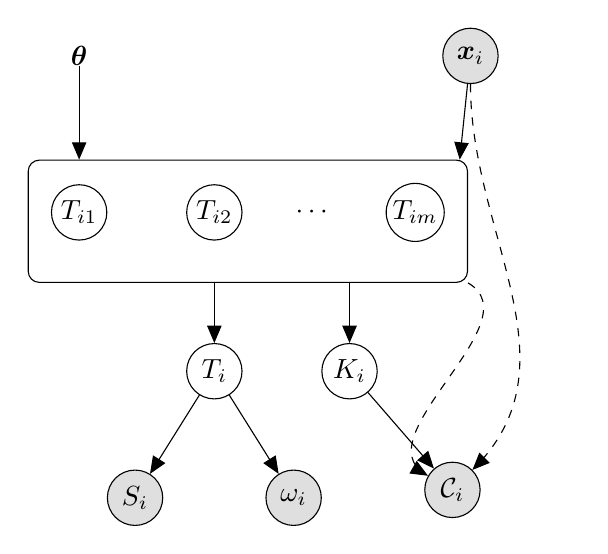
\begin{tikzpicture}[node distance=1.4cm]

  % ── Row 0: Parameters and covariates ──────────────────────────
  \node[const]                            (theta) {$\btheta$};
  \node[obs, right=4.5cm of theta]        (x)     {$\v{x}_i$};

  % ── Row 1: Component lifetimes (latent) ──────────────────────
  \node[latent, below=1.5cm of theta]     (T1)  {$T_{i1}$};
  \node[latent, right=of T1]              (T2)  {$T_{i2}$};
  \node[right=0.55cm of T2]              (Td)  {$\cdots$};
  \node[latent, right=0.55cm of Td]      (Tm)  {$T_{im}$};

  % Plate (visual grouping for component lifetimes)
  \plate[inner sep=8pt] {comp} {(T1)(T2)(Td)(Tm)} {};

  % ── Row 2: System-level latent variables ─────────────────────
  \node[latent, below=1.3cm of T2]        (Ti)  {$T_i$};
  \node[latent, right=of Ti]              (Ki)  {$K_i$};

  % ── Row 3: Observed quantities ───────────────────────────────
  \node[obs, below left=1.1cm and 0.5cm of Ti]   (Si)    {$S_i$};
  \node[obs, below right=1.1cm and 0.5cm of Ti]  (omega) {$\omega_i$};
  \node[obs, below right=1.0cm and 0.8cm of Ki]  (Ci)    {$\mathcal{C}_i$};

  % ── Solid edges (structural dependencies) ────────────────────

  % Parameters → plate
  \draw[->] (theta) -- (theta |- comp.north);

  % Covariates → plate
  \draw[->] (x) -- ([xshift=-3pt] comp.north east);

  % Component lifetimes → system lifetime
  \draw[->] (Ti |- comp.south) -- (Ti);

  % Component lifetimes → cause of failure
  \draw[->] (Ki |- comp.south) -- (Ki);

  % System lifetime → observation
  \edge {Ti} {Si,omega};

  % Cause of failure → candidate set
  \edge {Ki} {Ci};

  % ── Dashed edges (ignorable under C1–C2–C3) ─────────────────
  % With C_i placed to the lower-right, all three arrows into C_i
  % converge from different directions without any crossings.

  % x_i → candidate set: smooth curve from above-right
  \draw[->,dashed] (x) to[out=-90, in=45] (Ci);

  % Component lifetimes → candidate set (masking): from plate SE
  \draw[->,dashed] (comp.south east) to[out=-30, in=150] (Ci);

\end{tikzpicture}

\caption{Dependency model for the data generating process.
Shaded nodes are observed; open nodes are latent.
Solid arrows are structural dependencies; dashed arrows indicate
influences that are eliminated from the likelihood under C1--C2--C3.}
\label{fig:dep-model}
\end{figure}

\subsection{Example: Masked Data}
\label{sec:example-masked-data}

Table~\ref{tab:masked-data-example} shows an example of masked data for a
3-component series system with a right-censoring time $\tau = 5$.
Systems~5 and~6 are right-censored (their failures were not observed
before time $\tau$).
System~2 has a singleton candidate set, so its cause of failure is exactly
identified.
The remaining failed systems have candidate sets of size~2,
representing partial masking.

\begin{table}[ht]
\centering
\caption{Example of right-censored lifetime data with masked component
cause of failure for a 3-component series system ($\tau = 5$).}
\label{tab:masked-data-example}
\begin{tabular}{cccc}
\toprule
System & $s_i$ & $\omega_i$ & $c_i$ \\
\midrule
1 & 1.1 & $E$ & $\{1, 2\}$ \\
2 & 1.3 & $E$ & $\{2\}$ \\
3 & 2.6 & $E$ & $\{2, 3\}$ \\
4 & 3.7 & $E$ & $\{1, 3\}$ \\
5 & 5.0 & $R$ & $\emptyset$ \\
6 & 5.0 & $R$ & $\emptyset$ \\
\bottomrule
\end{tabular}
\end{table}


%=============================================================================
\section{The C1--C2--C3 Likelihood}
\label{sec:c1c2c3}
%=============================================================================

We now derive the likelihood contribution for an observation where the
system failure time is known but the component cause of failure is masked
by a candidate set.
The derivation below recapitulates and extends the classical
argument~\citep{miyakawa1984,Usher-1988} in a unified,
general form.

\subsection{Joint Distribution of \texorpdfstring{$T_i$, $K_i$, and $\mathcal{C}_i$}{Ti, Ki, and Ci}}
\label{sec:joint-tkc}

Our goal is to estimate $\btheta$ from observed data $D_i = (s_i, \omega_i, c_i, \v{x}_i)$.
When the system failure is observed ($\omega_i = E$), we observe the system
failure time $t_i$ and a candidate set $c_i$.
The joint pdf of the system lifetime $T_i$ and the candidate set
$\mathcal{C}_i$ is
\begin{equation}
\label{eq:joint-tc}
    f_{T_i, \mathcal{C}_i}(t_i, c_i; \btheta)
    = f_{T_i}(t_i; \btheta) \,
        \Pr_{\!\btheta}\{\mathcal{C}_i = c_i \mid T_i = t_i\}.
\end{equation}
While we assume the system lifetime pdf $f_{T_i}(t_i; \btheta)$ is known
(up to parameters), the conditional distribution
$\Pr_{\!\btheta}\{\mathcal{C}_i = c_i \mid T_i = t_i\}$ is generally
unknown---it depends on the diagnostic procedure, which we do not model.

Since $\mathcal{C}_i$ and $K_i$ are statistically dependent, we can
introduce $K_i$ into the analysis.
By Theorem~\ref{thm:joint-kt}, the joint pdf of $T_i$ and $K_i$ is
$f_{T_i, K_i}(t_i, j; \btheta) = h_j(t_i; \v{\theta}_j) \prod_{l=1}^m R_l(t_i; \v{\theta}_l)$.
The joint pdf of $T_i$, $K_i$, and $\mathcal{C}_i$ is therefore
\begin{equation}
\label{eq:joint-tkc}
    f_{T_i, K_i, \mathcal{C}_i}(t_i, j, c_i; \btheta)
    = h_j(t_i; \v{\theta}_j) \prod_{l=1}^m R_l(t_i; \v{\theta}_l)
        \cdot \Pr_{\!\btheta}\{\mathcal{C}_i = c_i \mid T_i = t_i, K_i = j\}.
\end{equation}
Marginalizing over $K_i$,
\begin{equation}
\label{eq:marginal-tc}
    f_{T_i, \mathcal{C}_i}(t_i, c_i; \btheta)
    = \prod_{l=1}^m R_l(t_i; \v{\theta}_l)
        \sum_{j=1}^m \biggl\{
            h_j(t_i; \v{\theta}_j) \,
            \Pr_{\!\btheta}\{\mathcal{C}_i = c_i \mid T_i = t_i, K_i = j\}
        \biggr\}.
\end{equation}

The unknown conditional probability
$\Pr_{\!\btheta}\{\mathcal{C}_i = c_i \mid T_i = t_i, K_i = j\}$
prevents direct use of this expression for likelihood-based inference.
We now introduce three conditions that successively simplify
Equation~\eqref{eq:marginal-tc} until the unknown masking distribution
drops out entirely.

\subsection{Condition 1: Candidate Set Contains the True Cause}
\label{sec:c1}

\begin{condition}[C1]
\label{cond:c1}
The candidate set $\mathcal{C}_i$ contains the index of the failed
component:
\begin{equation}
    \Pr_{\!\btheta}\{K_i \in \mathcal{C}_i\} = 1.
\end{equation}
\end{condition}

Condition~\ref{cond:c1} is the minimal requirement for the candidate set
to carry useful information about the failure cause: the true cause must
not be excluded.
In practice, real diagnostics work by \emph{narrowing down} from the
full component set---eliminating candidates that pass functional
checks---rather than constructing the candidate set from scratch.
Because exclusion of the true cause would require the diagnostic to
\emph{affirmatively misidentify} a functioning component as the sole
failure site, C1 holds whenever the diagnostic is competent in this
limited sense.

Two common diagnostic architectures illustrate the point.
First, automotive on-board diagnostics (OBD) fault codes are generated
by the failing module itself: a voltage exceedance or communication
timeout triggers the code, so the candidate set inherently includes the
true cause.
Second, hierarchical troubleshooting trees prune branches based on
pass/fail tests at each level; the true cause remains in the surviving
subtree at every step unless a test yields a false negative, which is a
calibration failure rather than a structural feature of the diagnostic.

In short, C1 asks for diagnostic \emph{competence}---not actively
wrong---rather than diagnostic \emph{precision}---exactly right.
Violating C1 is a pathological scenario (the diagnostic positively
excludes the failed component) that would undermine any analysis, masked
or otherwise.

\paragraph{What C1 buys.}
Under C1, if $j \notin c_i$ then
$\Pr_{\!\btheta}\{\mathcal{C}_i = c_i \mid T_i = t_i, K_i = j\} = 0$.
The summation in Equation~\eqref{eq:marginal-tc} therefore reduces from
$\{1, \ldots, m\}$ to $c_i$:
\begin{equation}
\label{eq:after-c1}
    f_{T_i, \mathcal{C}_i}(t_i, c_i; \btheta)
    = \prod_{l=1}^m R_l(t_i; \v{\theta}_l)
        \sum_{j \in c_i} \biggl\{
            h_j(t_i; \v{\theta}_j) \,
            \Pr_{\!\btheta}\{\mathcal{C}_i = c_i \mid T_i = t_i, K_i = j\}
        \biggr\}.
\end{equation}

\paragraph{What breaks without C1.}
Without C1, the summation must range over all $m$ components, and the
likelihood depends on the masking probabilities for components
\emph{outside} the candidate set.
This means the likelihood cannot be simplified without modeling the full
masking mechanism.

\subsection{Condition 2: Symmetric Masking Within the Candidate Set}
\label{sec:c2}

\begin{condition}[C2]
\label{cond:c2}
Given an observed system failure time $T_i = t_i$ and candidate set
$c_i$, the masking probability is the same regardless of which component
in $c_i$ is the true cause:
\begin{equation}
    \Pr_{\!\btheta}\{\mathcal{C}_i = c_i \mid T_i = t_i, K_i = j'\}
    = \Pr_{\!\btheta}\{\mathcal{C}_i = c_i \mid T_i = t_i, K_i = j\}
    \quad \text{for all } j, j' \in c_i.
\end{equation}
\end{condition}

Condition~\ref{cond:c2} is a requirement on the masking \emph{mechanism},
not merely on the observed data: it must hold for all candidate sets
$c_i$ that the mechanism can produce, not just the particular sets
realized in the sample.
When $|c_i| = 1$ (a singleton candidate set), C2 is satisfied
vacuously---the condition is non-trivial only when $|c_i| \geq 2$.
In words, C2 requires that the diagnostic does not
discriminate between components within the candidate set: given that a
particular candidate set is reported, no member of that set is favored
over another.
Symmetry arises naturally whenever masking is determined by
\emph{structural grouping}---subsystem, module, or physical
region---rather than by component-specific properties.
Components that share a group are indistinguishable to the diagnostic
precisely because the diagnostic operates at the group level.

Two additional examples reinforce this pattern.
In avionics maintenance, field technicians replace
\emph{line-replaceable units} (LRUs): every component inside the unit is
equally suspect because the diagnostic identified the unit, not the
component.
In industrial settings, SCADA monitoring systems report alarms at the
subsystem level---e.g., ``pump station fault''---without distinguishing
which element (motor, valve, seal) triggered the alarm; the candidate
set is the group, and all members are symmetric.

We acknowledge that C2 is the condition most likely to be violated in
practice, since partial diagnostic information can make one candidate
more plausible than another.
When asymmetry is suspected, a practical mitigation is to redefine
the candidate set at the finest resolution where symmetry still holds,
effectively trading a smaller candidate set for a valid application of
C2.

\paragraph{What C2 buys.}
Under C1 and C2, the masking probability
$\Pr_{\!\btheta}\{\mathcal{C}_i = c_i \mid T_i = t_i, K_i = j\}$
is constant for all $j \in c_i$ and can be factored out of the summation
in Equation~\eqref{eq:after-c1}:
\begin{equation}
\label{eq:after-c2}
    f_{T_i, \mathcal{C}_i}(t_i, c_i; \btheta)
    = \Pr_{\!\btheta}\{\mathcal{C}_i = c_i \mid T_i = t_i, K_i = j'\}
        \prod_{l=1}^m R_l(t_i; \v{\theta}_l)
        \sum_{j \in c_i} h_j(t_i; \v{\theta}_j),
\end{equation}
where $j'$ is any element of $c_i$.

\paragraph{What breaks without C2.}
Without C2, the masking probabilities remain inside the summation, coupling
the hazard contributions with component-specific masking weights.
The MLE then depends on the unknown masking probabilities, which must be
jointly estimated or modeled.

\subsection{Condition 3: Masking Independent of \texorpdfstring{$\btheta$}{theta}}
\label{sec:c3}

\begin{condition}[C3]
\label{cond:c3}
The masking probabilities, conditioned on the failure time and the
component cause of failure, do not depend on the system parameter
$\btheta$:
\begin{equation}
    \beta_i \coloneqq \Pr\{\mathcal{C}_i = c_i \mid T_i = t_i, K_i = j'\}
\end{equation}
is not a function of $\btheta$.
\end{condition}

Condition~\ref{cond:c3} states that the diagnostic procedure's behavior
is determined by factors external to the component lifetime parameters.
The masking probability $\beta_i$ may depend on the failure time (for
exact failures, where the diagnostic is performed at or near the observed
failure time), the diagnostician, the testing equipment, or other
covariates---but not on $\btheta$.
For censored observations, the diagnostic is performed at the inspection
time rather than at the unknown failure time; see
Remark~\ref{rem:diagnostic-timing} below.
The justification is fundamentally causal: the diagnostic tool was
designed and calibrated \emph{before} any failures were observed, so its
behavior cannot depend on the unknown $\btheta$ we are estimating.
For instance, OBD voltage thresholds are hard-coded at manufacture; a
vibration sensor's frequency band is set during installation.
Neither adapts to the lifetime parameters of the components it monitors.

Condition~\ref{cond:c3} is closely related to the concept of
\emph{ignorability} in the missing-data framework of
\citet{little2002statistical}.
In our setting, the ``missingness'' is the loss of exact cause
information through masking; C3 ensures that the masking mechanism is
\emph{ignorable} for likelihood-based inference, in the sense that the
conditional distribution of the candidate set need not be modeled when
maximizing the likelihood over~$\btheta$
\citep[see][Ch.~6]{little2002statistical}.

When covariates $\v{x}_i$ are present, C3 requires that the masking
probabilities do not depend on $\btheta$ \emph{given} the covariates
and failure time.
If the same covariates influence both the failure rate and the
diagnostic quality (e.g., an extreme operating environment that
accelerates failures and also degrades sensor accuracy), the
practitioner should verify that the masking mechanism remains
ignorable after conditioning on~$\v{x}_i$.

\paragraph{What C3 buys.}
Under C1, C2, and C3, the joint pdf becomes
\begin{equation}
\label{eq:after-c3}
    f_{T_i, \mathcal{C}_i}(t_i, c_i; \btheta)
    = \beta_i \prod_{l=1}^m R_l(t_i; \v{\theta}_l)
        \sum_{j \in c_i} h_j(t_i; \v{\theta}_j).
\end{equation}
When we view this as a function of $\btheta$ (with the data fixed),
$\beta_i$ is a constant multiplier that does not affect the location of
the maximum.
The likelihood contribution is therefore
\begin{equation}
\label{eq:likelihood-exact}
    L_i(\btheta) \propto \prod_{l=1}^m R_l(t_i; \v{\theta}_l)
        \sum_{j \in c_i} h_j(t_i; \v{\theta}_j).
\end{equation}

\paragraph{What breaks without C3.}
Without C3, the factor $\beta_i$ depends on $\btheta$ and cannot be
dropped.
The practitioner would need to model the dependence of the masking
mechanism on $\btheta$---a substantially harder problem that requires
additional data or assumptions about the diagnostic process.

\subsection{Real-World Example}
\label{sec:real-world-example}

To illustrate how the three conditions arise in practice, consider an
electronic device with three components arranged in a series
configuration.
Components~1 and~2 are on a shared circuit board, while component~3 is
separate.
A diagnostic tool isolates the failure to either the shared circuit
board or the individual component.
A more detailed board-level inspection sometimes pinpoints the specific
failed component; let $p \in (0,1)$ denote the probability that this
inspection succeeds.
The conditional probabilities for candidate sets are:
\[
\Pr\{\mathcal{C}_i = c_i \mid T_i = t_i, K_i = j\}
= \begin{cases}
    p   & \text{if } c_i = \{j\} \text{ and } j \in \{1, 2\}, \\
    1-p & \text{if } c_i = \{1, 2\} \text{ and } j \in \{1, 2\}, \\
    1   & \text{if } c_i = \{3\} \text{ and } j = 3, \\
    0   & \text{otherwise.}
\end{cases}
\]

This diagnostic tool satisfies all three conditions:
\begin{itemize}
    \item \textbf{C1}: The candidate set always contains the failed
    component---the tool correctly isolates failures to the correct
    subsystem (each possible candidate set contains the true cause).
    \item \textbf{C2}: For the candidate set $\{1, 2\}$, the masking
    probability is the same whether component~1 or component~2 failed
    (both equal~$1-p$).
    For singleton candidate sets $\{1\}$ or $\{2\}$,
    Condition~\ref{cond:c2} is satisfied trivially.
    \item \textbf{C3}: The masking probabilities depend only on the
    diagnostic tool (through~$p$) and not on the component lifetime
    parameters~$\btheta$.
\end{itemize}

The parameter $p > 0$ is essential for identifiability: when the
board-level inspection never succeeds ($p = 0$), components~1 and~2
always appear together in every candidate set and their individual
parameters cannot be separated---see
Section~\ref{sec:identifiability} for a detailed discussion.
Any $p > 0$ ensures that some observations produce singleton candidate
sets $\{1\}$ or $\{2\}$, providing the information needed to
distinguish the two components.

According to \citet{guess1991}, many industrial diagnostic scenarios
naturally satisfy these conditions, reinforcing the practical
applicability of the framework.

\subsection{Censored Observations with Candidate Sets}
\label{sec:censored-masked}

The C1--C2--C3 derivation in Sections~\ref{sec:c1}--\ref{sec:c3} applies to
any observation where a failure is known to have occurred.
Equation~\eqref{eq:after-c3} gives the joint density of the failure time
and candidate set at a \emph{specific} time~$t_i$.
For left-censored and interval-censored observations, the failure time
is not known exactly, so we integrate over the admissible range.

\begin{remark}[Diagnostic timing and the masking probability]
\label{rem:diagnostic-timing}
For an exact failure, the diagnostic may be performed at or near the
observed failure time~$t_i$, so $\beta_i = \beta(t_i)$ is evaluated at a
known point and is a scalar constant in the likelihood.
For censored observations, the diagnostic is performed at the inspection
time---when the system's failed state is discovered---not at the unknown
failure time~$T_i$.
(For interval-censored observations, this is typically the later
inspection time~$b_i$, at which the failure is first detected.)
The masking probability is therefore
$\beta_i = \Pr\{\mathcal{C}_i = c_i \mid \text{system failed by
inspection},\, K_i = j'\}$,
which does not depend on the integration variable~$t$.
This is the natural model: inspectors diagnose the current state at
inspection time and do not have access to the unknown failure time.
Consequently, $\beta_i$ factors out of the integrals in the left-censored
and interval-censored likelihood contributions below, and by
Condition~\ref{cond:c3} it does not depend on $\btheta$, so it may be
dropped.
\end{remark}

\begin{theorem}[Left-censored likelihood contribution under C1--C2--C3]
\label{thm:left-censored}
Under Conditions~\ref{cond:c1}--\ref{cond:c3}, if the $i$th system is
known to have failed by time $\tau_i$ with candidate set $c_i$, the
likelihood contribution is
\begin{equation}
\label{eq:left-censored}
    L_i(\btheta) \propto
    \int_0^{\tau_i}
    \sum_{j \in c_i} h_j(t; \v{\theta}_j)
    \prod_{l=1}^m R_l(t; \v{\theta}_l) \, dt.
\end{equation}
\end{theorem}

\begin{proof}
By Equation~\eqref{eq:after-c3}, the joint density of the failure time
and candidate set at time~$t$ is
$\beta_i \sum_{j \in c_i} h_j(t; \v{\theta}_j)
\prod_{l=1}^m R_l(t; \v{\theta}_l)$.
Since the failure time is known only to satisfy $T_i \leq \tau_i$, we
integrate over $t \in (0, \tau_i]$.
As noted in Remark~\ref{rem:diagnostic-timing}, the diagnostic is
performed at inspection time, so $\beta_i$ does not depend on the
integration variable~$t$ and factors out of the integral.
By Condition~\ref{cond:c3}, $\beta_i$ does not depend on $\btheta$
either, so it is a constant factor that may be dropped.
\end{proof}

\begin{theorem}[Interval-censored likelihood contribution under C1--C2--C3]
\label{thm:interval-censored}
Under Conditions~\ref{cond:c1}--\ref{cond:c3}, if the $i$th system
failed in the interval $(a_i, b_i]$ with candidate set $c_i$, the
likelihood contribution is
\begin{equation}
\label{eq:interval-censored}
    L_i(\btheta) \propto
    \int_{a_i}^{b_i}
    \sum_{j \in c_i} h_j(t; \v{\theta}_j)
    \prod_{l=1}^m R_l(t; \v{\theta}_l) \, dt.
\end{equation}
\end{theorem}

\begin{proof}
The argument is identical to the proof of
Theorem~\ref{thm:left-censored}---with $\beta_i$ again constant by the
diagnostic-timing reasoning of Remark~\ref{rem:diagnostic-timing}---but
with the integration domain restricted to $(a_i, b_i]$.
\end{proof}

\begin{remark}
When no cause information is available ($c_i = \{1, \ldots, m\}$), these
contributions reduce to the standard censored-data forms.
For the left-censored case,
\[
    \int_0^{\tau_i}
    \sum_{j=1}^m h_j(t; \v{\theta}_j)
    \prod_{l=1}^m R_l(t; \v{\theta}_l) \, dt
    = \int_0^{\tau_i} f_{T_i}(t; \btheta) \, dt
    = 1 - \prod_{j=1}^m R_j(\tau_i; \v{\theta}_j),
\]
by Equation~\eqref{eq:sys-pdf-convenient}.
Similarly, the interval-censored contribution reduces to
\[
    \prod_{j=1}^m R_j(a_i; \v{\theta}_j)
    - \prod_{j=1}^m R_j(b_i; \v{\theta}_j).
\]
\end{remark}

\subsection{Combined Likelihood}
\label{sec:combined-likelihood}

We now assemble the full likelihood from the individual contributions
(Equation~\eqref{eq:likelihood-exact},
Theorems~\ref{thm:left-censored}--\ref{thm:interval-censored}, and the
right-censored case from Theorem~\ref{thm:sys-reliability}).
Let $\mathcal{E} = \{i : \omega_i = E\}$,
$\mathcal{R} = \{i : \omega_i = R\}$,
$\mathcal{L} = \{i : \omega_i = L\}$, and
$\mathcal{I} = \{i : \omega_i = I\}$ denote the
index sets of observations that are exact failures, right-censored,
left-censored, and interval-censored, respectively.

\begin{theorem}[Likelihood under C1--C2--C3]
\label{thm:likelihood-contribution}
Under Conditions~\ref{cond:c1}--\ref{cond:c3}, the likelihood for the
observed data $D = \{D_1, \ldots, D_n\}$ is
\begin{align}
\label{eq:combined-likelihood}
    L(\btheta) \;\propto\;\;
    &\prod_{i \in \mathcal{E}}
        \biggl[\prod_{l=1}^m R_l(t_i; \v{\theta}_l)
        \cdot \sum_{j \in c_i} h_j(t_i; \v{\theta}_j)\biggr]
    \;\prod_{i \in \mathcal{R}}
        \biggl[\prod_{j=1}^m R_j(\tau_i; \v{\theta}_j)\biggr]
        \notag \\
    &\times
    \prod_{i \in \mathcal{L}}
        \biggl[\int_0^{\tau_i}
        \sum_{j \in c_i} h_j(t; \v{\theta}_j)
        \prod_{l=1}^m R_l(t; \v{\theta}_l) \, dt\biggr]
    \;\prod_{i \in \mathcal{I}}
        \biggl[\int_{a_i}^{b_i}
        \sum_{j \in c_i} h_j(t; \v{\theta}_j)
        \prod_{l=1}^m R_l(t; \v{\theta}_l) \, dt\biggr].
\end{align}
\end{theorem}

\begin{proof}
Each factor follows from the corresponding individual result:
the exact-failure contribution from Equation~\eqref{eq:likelihood-exact},
the right-censored contribution from
Theorem~\ref{thm:sys-reliability},
the left-censored contribution from
Theorem~\ref{thm:left-censored}, and the interval-censored contribution
from Theorem~\ref{thm:interval-censored}.
Independence across systems gives the product.
\end{proof}

\subsection{Identifiability}
\label{sec:identifiability}

Before addressing identifiability within our framework, we note the
classical competing risks result of \citet{tsiatis1975}: without the
component independence assumption (Remark~\ref{rem:independence}),
the marginal component lifetime distributions are not identifiable from
system lifetime data alone---even with complete observation of the
failure cause.
Our framework inherits identifiability from the independence assumption,
which allows the system reliability to factor as a product of component
reliabilities (Theorem~\ref{thm:sys-reliability}).
Given independence, the identifiability question reduces to whether the
observed candidate sets provide enough information to separate the
component parameters.

\begin{definition}[Candidate-set separability]
\label{def:separability}
Let $\mathcal{S}$ denote the collection of candidate sets that occur
with positive probability under the masking mechanism.
We say the masking mechanism is \emph{separating} if, for every pair
of distinct components $j \neq j'$, there exists a candidate set
$c \in \mathcal{S}$ such that $j \in c$ and $j' \notin c$.
When this condition fails for some pair $(j, j')$---that is,
$j \in c \iff j' \in c$ for every $c \in \mathcal{S}$---we say $j$
and $j'$ are \emph{diagnostically confounded}.
\end{definition}

The following theorem shows that separability is the key condition
governing identifiability under C1--C2--C3.

\begin{theorem}[Identifiability under C1--C2--C3]
\label{thm:identifiability}
Let $h_j(t; \v{\theta}_j)$ be the hazard function for component~$j$,
where $\v{\theta} = (\v{\theta}_1, \ldots, \v{\theta}_m) \in \Theta
\subseteq \mathbb{R}^p$ is the full parameter vector, and suppose
each component family is individually identifiable: $h_j(\cdot\,;
\v{\theta}_j) = h_j(\cdot\,; \v{\theta}_j')$ for all $t > 0$ implies
$\v{\theta}_j = \v{\theta}_j'$.
Under C1--C2--C3:
\begin{enumerate}
    \item[\emph{(a)}] \textbf{Necessary condition.}
    If components $j$ and $j'$ are diagnostically confounded
    (Definition~\ref{def:separability}), then $\v{\theta}_j$ and
    $\v{\theta}_{j'}$ are not separately identifiable from the
    observed-data likelihood.
    Specifically, any reparametrization preserving
    $h_j(t; \v{\theta}_j) + h_{j'}(t; \v{\theta}_{j'})$ for all
    $t > 0$ yields the same likelihood value.

    \item[\emph{(b)}] \textbf{Sufficient condition.}
    If the masking mechanism is separating
    (Definition~\ref{def:separability}), and at least some
    observations are exact failures (type~$E$), then the parameter
    vector $\v{\theta}$ is identifiable for any parametric family
    whose hazard functions $\{h_1, \ldots, h_m\}$ are linearly
    independent over $(0, \infty)$.
\end{enumerate}
\end{theorem}

\begin{proof}
\emph{Part~(a).}
Suppose $j \in c \iff j' \in c$ for every $c \in \mathcal{S}$.
Then in every exact-failure likelihood contribution
$R(t_i) \sum_{l \in c_i} h_l(t_i)$
(Equation~\ref{eq:likelihood-exact}),
the hazards $h_j$ and $h_{j'}$ appear as a sum
$h_j(t_i) + h_{j'}(t_i)$ wherever they appear at all.
The survival factor
$R(t_i) = \exp\bigl(-\sum_l H_l(t_i)\bigr)$ likewise depends on
$H_j(t_i) + H_{j'}(t_i)$ only through their sum.
The same holds for right-, left-, and interval-censored
contributions (Table~\ref{tab:likelihood-contributions}),
since all involve $R(t)$ and $\sum_{l \in c} h_l(t)$.
Hence the likelihood $L(\v{\theta})$ depends on $\v{\theta}_j$ and
$\v{\theta}_{j'}$ only through the sum $h_j + h_{j'}$, and any
reallocation preserving this sum leaves $L$ unchanged.

\emph{Part~(b).}
Suppose the masking mechanism is separating and let
$\v{\theta} \neq \v{\theta}'$ with $L(\v{\theta}) = L(\v{\theta}')$
for all data sets.
Then in particular, for a data set consisting of a single exact failure
at time~$t$ with candidate set~$c$, the log-likelihood equality gives
\begin{equation}
\label{eq:ident-proof}
    -\sum_l H_l(t) + \log \sum_{j \in c} h_j(t)
    = -\sum_l H_l'(t) + \log \sum_{j \in c} h_j'(t)
\end{equation}
for all $t > 0$ and all $c \in \mathcal{S}$, where
$h_j = h_j(\cdot\,; \v{\theta}_j)$ and
$h_j' = h_j(\cdot\,; \v{\theta}_j')$.
Differentiating~\eqref{eq:ident-proof} with respect to~$t$ for two
candidate sets $c_1, c_2 \in \mathcal{S}$ with
$j \in c_1$, $j \notin c_2$ (which exist by separability) and
subtracting yields a relation that isolates the contribution of
component~$j$.
Specifically, from the survival terms we obtain
$\sum_l h_l(t) = \sum_l h_l'(t)$, and from candidate sets separating
$j$ we obtain that $h_j(t) = h_j'(t)$ for all $t > 0$ whenever
$h_1, \ldots, h_m$ are linearly independent.
By the individual identifiability assumption,
$\v{\theta}_j = \v{\theta}_j'$ for each~$j$.
\end{proof}

Part~(a) states that diagnostically confounded components are
fundamentally unresolvable: the likelihood surface has a ridge along
all reparametrizations of the confounded pair, producing an infinite
family of equivalent maximizers rather than a unique MLE.
Part~(b) provides a checkable condition: the analyst needs only
inspect the candidate-set structure~$\mathcal{S}$ to verify separability.

\begin{remark}[Linear independence of hazard functions]
\label{rem:linear-independence}
The linear independence condition in
Theorem~\ref{thm:identifiability}(b) holds generically for all
families in Table~\ref{tab:distributions}.
The Weibull hazard $h_j(t) \propto t^{k_j - 1}$ with distinct
shapes $k_j$ yields linearly independent power functions.
For the exponential family ($k_j = 1$ for all~$j$), the hazards
are constant and hence linearly \emph{dependent}; in this case,
separability of the candidate sets carries the full burden of
identifiability.
For families with identical functional form across components
(e.g., exponential or homogeneous Weibull), identifiability requires
that the candidate-set matrix
$C \in \{0,1\}^{|\mathcal{S}| \times m}$---whose rows are the
indicator vectors of the candidate sets in $\mathcal{S}$---has full
column rank~$m$.
This is strictly stronger than separability
(which requires only that no two columns of~$C$ are identical) but
is guaranteed when $\mathcal{S}$ includes a singleton $\{j\}$ for
each component~$j$.
\end{remark}

\paragraph{Remediation of non-identifiability.}
When components~$j$ and~$j'$ are diagnostically confounded, three
strategies are available:
\begin{enumerate}
    \item \textbf{Collapse into a super-component.}
    Replace the always-grouped components with a single composite
    component whose hazard is $h_j + h_{j'}$.
    This reduces the parameter count and restores identifiability at the
    cost of losing individual component resolution.
    \item \textbf{Impose equality constraints.}
    Assume the grouped components share identical parameter
    values ($\v{\theta}_j = \v{\theta}_{j'}$), splitting the combined
    hazard equally.
    This is appropriate when the components are physically
    interchangeable (e.g., identical capacitors on the same circuit
    board).
    \item \textbf{Bayesian regularization.}
    Place informative priors on $\v{\theta}_j$ and $\v{\theta}_{j'}$ to
    obtain a proper posterior even when the likelihood surface is flat.
    The posterior concentrates as additional diagnostic information becomes
    available, so the prior penalty vanishes asymptotically.
\end{enumerate}
In each case, the practitioner should examine the candidate-set
structure of the data before fitting the model.
Convergence difficulties in numerical optimization (e.g., failure to
converge within a maximum number of iterations) may signal that the
separability condition of Definition~\ref{def:separability} is
violated or nearly violated.


%=============================================================================
\section{Maximum Likelihood Estimation}
\label{sec:mle}
%=============================================================================

Maximum likelihood estimation (MLE) finds the parameter values that
maximize the likelihood of the observed
data~\citep{bain1992,casella2002statistical}.
A maximum likelihood estimate $\hat{\btheta}$ satisfies
\begin{equation}
\label{eq:mle-def}
    L(\hat{\btheta}) = \max_{\btheta \in \bomega} L(\btheta).
\end{equation}

For computational efficiency, we work with the log-likelihood.

\begin{theorem}[Log-likelihood]
\label{thm:log-likelihood}
Under Conditions~\ref{cond:c1}--\ref{cond:c3}, the log-likelihood for
the masked data model is
\begin{equation}
\label{eq:log-likelihood}
    \ell(\btheta) = \ell_E(\btheta) + \ell_R(\btheta)
    + \ell_L(\btheta) + \ell_I(\btheta),
\end{equation}
where
\begin{align}
\label{eq:log-likelihood-E}
    \ell_E(\btheta)
    &= \sum_{i \in \mathcal{E}} \biggl[
        \sum_{j=1}^m \log R_j(t_i; \v{\theta}_j)
        + \log\biggl(\sum_{j \in c_i} h_j(t_i; \v{\theta}_j)\biggr)
    \biggr], \\[6pt]
\label{eq:log-likelihood-R}
    \ell_R(\btheta)
    &= \sum_{i \in \mathcal{R}}
        \sum_{j=1}^m \log R_j(\tau_i; \v{\theta}_j), \\[6pt]
\label{eq:log-likelihood-L}
    \ell_L(\btheta)
    &= \sum_{i \in \mathcal{L}}
        \log\biggl[\int_0^{\tau_i}
        \sum_{j \in c_i} h_j(t; \v{\theta}_j)
        \prod_{l=1}^m R_l(t; \v{\theta}_l) \, dt\biggr], \\[6pt]
\label{eq:log-likelihood-I}
    \ell_I(\btheta)
    &= \sum_{i \in \mathcal{I}}
        \log\biggl[\int_{a_i}^{b_i}
        \sum_{j \in c_i} h_j(t; \v{\theta}_j)
        \prod_{l=1}^m R_l(t; \v{\theta}_l) \, dt\biggr].
\end{align}
\end{theorem}

\begin{proof}
Taking logarithms in Theorem~\ref{thm:likelihood-contribution} and
using $\log \prod = \sum \log$ gives the result directly.
\end{proof}

\begin{remark}[Common special case]
\label{rem:common-case}
When only exact failures and right-censored observations are present
($\mathcal{L} = \mathcal{I} = \emptyset$), the log-likelihood reduces to
$\ell(\btheta) = \ell_E(\btheta) + \ell_R(\btheta)$
(Equations~\eqref{eq:log-likelihood-E}
and~\eqref{eq:log-likelihood-R}).
This is the form used in most companion papers.
\end{remark}

\subsection{Score Equations}
\label{sec:score-equations}

The MLE is found by solving the score equations
\begin{equation}
\label{eq:score}
    \frac{\partial}{\partial \theta_{j,r}} \ell(\btheta) = 0,
\end{equation}
for each parameter $\theta_{j,r}$ (the $r$th element of the $j$th
component's parameter vector).
In general, these equations do not admit closed-form solutions and must
be solved numerically using methods such as Newton--Raphson or
quasi-Newton algorithms~\citep{nocedal2006numerical,byrd1995}.

\subsection{Asymptotic Properties}
\label{sec:asymptotic-properties}

Under standard regularity conditions (which must be verified for each
specific distribution family)---including identifiability,
smoothness of the log-likelihood, and the true parameter lying in the
interior of the parameter space---the MLE is consistent, asymptotically normal, and
asymptotically efficient~\citep{casella2002statistical,lehmann1998theory}.
That is, as $n \to \infty$,
$\hat{\btheta} \xrightarrow{p} \btheta_0$ (the true parameter) and
$\sqrt{n}(\hat{\btheta} - \btheta_0) \xrightarrow{d}
\mathcal{N}(\v{0}, \mathcal{I}^{-1}(\btheta_0))$,
where $\mathcal{I}(\btheta_0)$ is the per-observation Fisher information matrix.
For finite samples, these asymptotic approximations may be inaccurate,
and bootstrap methods (e.g., the bias-corrected and accelerated
method~\citep{efron1987better,efron1994introduction}) provide a
nonparametric alternative for constructing confidence intervals.

\subsection{General Recipe for Practitioners}
\label{sec:recipe}

Given a hazard function $h_j(t; \v{\theta}_j, \v{x}_i)$ for each
component, the practitioner applies the framework as follows:
\begin{enumerate}
    \item \textbf{Specify} the component hazard functions
    $h_j(t; \v{\theta}_j, \v{x}_i)$ and compute
    $R_j = \exp\!\bigl(-\int_0^t h_j \, du\bigr)$
    (analytically if possible, numerically otherwise).
    \item \textbf{Substitute} the component-specific $R_j$ and $h_j$ into
    the log-likelihood (Equation~\eqref{eq:log-likelihood}).
    \item \textbf{Differentiate} the log-likelihood with respect to each
    parameter to obtain the score equations.
    \item \textbf{Solve} the score equations numerically (e.g., using
    L-BFGS-B~\citep{byrd1995} or Newton--Raphson) to obtain
    $\hat{\btheta}$.
    \item \textbf{Construct confidence intervals} using the observed
    Fisher information or bootstrap resampling.
\end{enumerate}

Section~\ref{sec:families} provides hazard functions for five common
parametric families, enabling immediate application of this recipe.

\subsection{Worked Example: Exponential Components}
\label{sec:worked-example}

We illustrate the recipe using the data in
Table~\ref{tab:masked-data-example} ($m = 3$ components, $n = 6$
observations) with Exponential component lifetimes.
For Exponential components, $R_j(t; \lambda_j) = e^{-\lambda_j t}$
and $h_j(t; \lambda_j) = \lambda_j$, where $\lambda_j > 0$ is the
failure rate of the $j$th component.

Since the data contain only exact failures and right-censored
observations, the log-likelihood is
$\ell = \ell_E + \ell_R$ (Remark~\ref{rem:common-case}).
For Exponential components, $\log R_j(t; \lambda_j) = -\lambda_j t$
and $h_j(t; \lambda_j) = \lambda_j$, so the two contributions are:
\begin{align}
\label{eq:ll-exp-E}
    \ell_E
    &= \sum_{i \in \mathcal{E}} \biggl[
        -(\lambda_1 + \lambda_2 + \lambda_3) \, t_i
        + \log\biggl(\sum_{j \in c_i} \lambda_j\biggr)
    \biggr], \\[4pt]
\label{eq:ll-exp-R}
    \ell_R
    &= \sum_{i \in \mathcal{R}}
        \bigl[-(\lambda_1 + \lambda_2 + \lambda_3) \, \tau_i\bigr].
\end{align}
Substituting the data from Table~\ref{tab:masked-data-example}
(with $T_{\mathrm{total}} = \sum_{i=1}^n s_i = 18.7$),
the combined log-likelihood is
\begin{equation}
\label{eq:ll-exponential-explicit}
    \ell = -18.7 \, (\lambda_1 + \lambda_2 + \lambda_3)
    + \log(\lambda_1 + \lambda_2)
    + \log(\lambda_2)
    + \log(\lambda_2 + \lambda_3)
    + \log(\lambda_1 + \lambda_3).
\end{equation}
The score equations $\partial \ell / \partial \lambda_j = 0$ are
\begin{align}
    \frac{\partial \ell}{\partial \lambda_1}
    &= -18.7
        + \frac{1}{\lambda_1 + \lambda_2}
        + \frac{1}{\lambda_1 + \lambda_3} = 0,
        \label{eq:score-exp-1} \\
    \frac{\partial \ell}{\partial \lambda_2}
    &= -18.7
        + \frac{1}{\lambda_1 + \lambda_2}
        + \frac{1}{\lambda_2}
        + \frac{1}{\lambda_2 + \lambda_3} = 0,
        \label{eq:score-exp-2} \\
    \frac{\partial \ell}{\partial \lambda_3}
    &= -18.7
        + \frac{1}{\lambda_2 + \lambda_3}
        + \frac{1}{\lambda_1 + \lambda_3} = 0.
        \label{eq:score-exp-3}
\end{align}
Subtracting~\eqref{eq:score-exp-3} from~\eqref{eq:score-exp-1} gives
$1/(\lambda_1 + \lambda_2) = 1/(\lambda_2 + \lambda_3)$, so
$\hat\lambda_1 = \hat\lambda_3$.
Setting $\alpha = \lambda_1 = \lambda_3$ and $\beta = \lambda_2$,
the system reduces to two equations whose solution is
\begin{equation}
    \hat\lambda_1 = \hat\lambda_3
    = \frac{7 - \sqrt{17}}{74.8} \approx 0.0385, \qquad
    \hat\lambda_2
    = \frac{1 + \sqrt{17}}{37.4} \approx 0.1370.
\end{equation}
The total system failure rate is
$\hat\lambda_1 + \hat\lambda_2 + \hat\lambda_3 = 4/18.7 \approx 0.2139$,
which equals the number of observed failures divided by the total
exposure time---a general property of the Exponential MLE.
The masking affects only the \emph{allocation} of hazard across
components, not the total.

Component~2 has the highest estimated failure rate, consistent with
its appearance in three of the four failure candidate sets (including
a singleton).
Components~1 and~3 have equal rates by symmetry: each appears in
exactly two candidate sets, with identical structure after relabeling.


%=============================================================================
\section{Common Hazard Function Specifications}
\label{sec:families}
%=============================================================================

Table~\ref{tab:distributions} lists hazard functions for five standard
parametric families, illustrating how the general framework specializes.
Any hazard function $h_j(t; \v{\theta}_j)$ satisfying the regularity
conditions of Section~\ref{sec:asymptotic-properties} can be used; the
named families below are common starting points.

\begin{table}[ht]
\centering
\caption{Common hazard function specifications.
The hazard function $h_j$ is the primary specification; the reliability
function $R_j$ and density $f_j$ are derived via
Equations~\eqref{eq:rel-from-haz}--\eqref{eq:pdf-from-haz}.}
\label{tab:distributions}
\footnotesize
\renewcommand{\arraystretch}{1.6}
\begin{tabular}{@{}lcccc@{}}
\toprule
\textbf{Family} & $h_j(t; \v{\theta}_j)$ & $R_j(t; \v{\theta}_j)$
    & $f_j(t; \v{\theta}_j)$ & \textbf{Parameters} \\
\midrule
Exponential
    & $\lambda_j$
    & $e^{-\lambda_j t}$
    & $\lambda_j e^{-\lambda_j t}$
    & $\lambda_j > 0$ \\
Weibull
    & $\dfrac{k_j}{\lambda_j}\Bigl(\dfrac{t}{\lambda_j}\Bigr)^{k_j - 1}$
    & $e^{-(t/\lambda_j)^{k_j}}$
    & $\dfrac{k_j}{\lambda_j}\Bigl(\dfrac{t}{\lambda_j}\Bigr)^{k_j - 1}
        e^{-(t/\lambda_j)^{k_j}}$
    & $k_j, \lambda_j > 0$ \\
Pareto
    & $\dfrac{\alpha_j}{t}$
    & $\Bigl(\dfrac{x_{\min,j}}{t}\Bigr)^{\!\alpha_j}$
    & $\dfrac{\alpha_j \, x_{\min,j}^{\alpha_j}}{t^{\alpha_j + 1}}$
    & $\alpha_j, x_{\min,j} > 0$; $t \geq x_{\min,j}$ \\
Log-normal
    & $\dfrac{\phi\bigl(\frac{\log t - \mu_j}{\sigma_j}\bigr)}
        {\sigma_j \, t \bigl[1 - \Phi\bigl(\frac{\log t - \mu_j}{\sigma_j}\bigr)\bigr]}$
    & $1 - \Phi\!\Bigl(\dfrac{\log t - \mu_j}{\sigma_j}\Bigr)$
    & $\dfrac{1}{\sigma_j t}\,
        \phi\!\Bigl(\dfrac{\log t - \mu_j}{\sigma_j}\Bigr)$
    & $\mu_j \in \mathbb{R}$, $\sigma_j > 0$ \\
Gamma\footnotemark
    & $\dfrac{f_j(t; \v{\theta}_j)}{R_j(t; \v{\theta}_j)}$
    & $1 - \dfrac{\gamma(\alpha_j, \beta_j t)}{\Gamma(\alpha_j)}$
    & $\dfrac{\beta_j^{\alpha_j}}{\Gamma(\alpha_j)} \,
        t^{\alpha_j - 1} e^{-\beta_j t}$
    & $\alpha_j, \beta_j > 0$ \\
\bottomrule
\end{tabular}
\end{table}
\footnotetext{The Gamma hazard function has no elementary closed form;
it is expressed here via its definition $h_j = f_j / R_j$.}

In Table~\ref{tab:distributions}, $\Phi(\cdot)$ and $\phi(\cdot)$ denote
the standard normal CDF and pdf, respectively; $\gamma(\cdot, \cdot)$ is the
lower incomplete gamma function; and $\Gamma(\cdot)$ is the gamma function.
For distributions with parameter-dependent support (e.g., the Pareto
distribution with $t \geq x_{\min,j}$), the system support is
$t \geq \max_j x_{\min,j}$, and the product formula for system reliability
(Theorem~\ref{thm:sys-reliability}) must be applied only on this common
support.

\begin{remark}[Covariate-dependent hazards]
\label{rem:covariate-hazards}
The hazard function $h_j(t; \v{\theta}_j, \v{x}_i)$ may incorporate
observation-level covariates $\v{x}_i$. A common special case is the
proportional hazards specification
$h_j(t; \v{\theta}_j, \v{x}_i) = h_{0,j}(t; \v{\theta}_j)
\exp(\v{x}_i^\top \v{\beta}_j)$,
where $h_{0,j}$ is a baseline hazard from any family in
Table~\ref{tab:distributions} and $\v{\beta}_j$ is a
component-specific regression coefficient vector.
The likelihood expressions of Section~\ref{sec:c1c2c3} remain valid;
only the functional form of $h_j$ changes.
\end{remark}

\begin{remark}[Nested models within a family]
\label{rem:nested-models}
Several families in Table~\ref{tab:distributions} admit natural
hierarchies of nested sub-models.
For instance, the Weibull family contains a common-shape reduction
($m + 1$ parameters) in which the system lifetime is itself Weibull,
and a further exponential specialization ($m$ parameters) with fully
analytical inference.
These nestings enable formal model selection via likelihood ratio
tests, AIC, or BIC.
A detailed treatment---including simulation studies quantifying when
a reduced model is appropriate---is given
in~\citet{towell2025model-selection}.
\end{remark}


%=============================================================================
\section{Discussion}
\label{sec:discussion}
%=============================================================================

\subsection{What the Framework Enables}
\label{sec:what-enables}

The hazard-function-based likelihood framework developed in this paper
provides a foundation for a family of distribution-specific companion
papers.
Each companion paper can focus on a specific parametric family---for
example, Weibull~\citep{towell2025weibull-series} or
Exponential~\citep{towell2025exponential-series}---deriving
closed-form score equations and Fisher information matrices, conducting
simulation studies to assess MLE performance under varying masking and
censoring scenarios, and developing specialized software packages, all
while citing the present work for the general theory.
The layered software stack described in
Section~\ref{sec:software}---from component specification
(\texttt{flexhaz}) through series composition
(\texttt{serieshaz}) to masked-data likelihood
(\texttt{maskedhaz})---demonstrates this modularity:
new component distributions inherit the full estimation pipeline
without distribution-specific likelihood code.

\subsection{Relaxation of Conditions}
\label{sec:relaxations}

The three conditions (C1--C2--C3) provide a clean mathematical framework,
but practitioners may encounter situations where one or more conditions
are violated.
We briefly sketch what happens in each case:

\begin{itemize}
    \item \textbf{Relaxing C1} (candidate set may not contain the true
    cause): The summation in the likelihood cannot be restricted to
    $c_i$; the full component set must be considered, along with a model
    for the probability that the true cause is excluded from the candidate
    set.
    This introduces additional nuisance parameters.

    \item \textbf{Relaxing C2} (asymmetric masking): The masking
    probabilities $\Pr\{\mathcal{C}_i = c_i \mid T_i = t_i, K_i = j\}$
    remain inside the summation and couple with the component hazards.
    The MLE depends on the relative masking probabilities, which must
    be estimated or modeled.

    \item \textbf{Relaxing C3} (masking depends on $\btheta$): The
    factor $\beta_i$ cannot be dropped from the likelihood, and the MLE
    must account for the dependence of the masking mechanism on the
    lifetime parameters.
    This leads to a more complex joint estimation problem.
\end{itemize}

Detailed treatment of these relaxations is beyond the scope of this
paper and is deferred to future work.

\subsection{Computational Considerations}
\label{sec:computational}

Several practical issues arise when applying the framework:

\begin{itemize}
    \item \textbf{Local optima.}
    The log-likelihood surface may be multimodal, particularly under
    heavy masking or censoring.
    Multiple random starting points for the numerical optimizer are
    recommended.

    \item \textbf{Convergence.}
    Failure to converge within a reasonable number of iterations may
    indicate identifiability issues for the given data set.
    Such cases should be flagged rather than silently discarded.

    \item \textbf{Boundary constraints.}
    Many lifetime distributions have positivity constraints on parameters.
    Constrained optimization methods such as L-BFGS-B~\citep{byrd1995}
    or reparameterization (e.g., optimizing over log-scale parameters)
    can enforce these constraints.
\end{itemize}

\subsection{Software Ecosystem}
\label{sec:software}

The framework developed in this paper is implemented as a layered
software stack in the R statistical computing
environment~\citep{towell2025flexhaz,towell2025serieshaz,towell2025maskedhaz}.
At the base, the \texttt{flexhaz}
package~\citep{towell2025flexhaz} provides a hazard-function-first
abstraction for individual component lifetime distributions: each
distribution is specified by its hazard function, from which the
cumulative hazard, reliability, density, and random sampling follow
(cf.\ Equations~\eqref{eq:cumhaz-def}--\eqref{eq:pdf-from-haz}).
The \texttt{serieshaz} package~\citep{towell2025serieshaz}
composes components into series system distributions using hazard
additivity (Theorem~\ref{thm:sys-hazard}), with a parameter layout
that maps the global vector~$\btheta$ to component-specific
subvectors~$\v{\theta}_j$.
The \texttt{maskedhaz}
package~\citep{towell2025maskedhaz} implements the C1--C2--C3
log-likelihood (Theorem~\ref{thm:log-likelihood}) for all four
observation types (exact, right-censored, left-censored, and
interval-censored), taking arbitrary component hazard closures as
input.
Together these packages enable practitioners to apply the recipe of
Section~\ref{sec:recipe} with any component distribution in the
\texttt{flexhaz} ecosystem, without writing distribution-specific
likelihood code.

For Weibull component lifetimes specifically, the
\texttt{wei.series.md.c1.c2.c3}
package~\citep{towell2023weibull} provides closed-form score
vectors and Fisher information, along with bootstrap confidence
interval construction~\citep{towell2023algebraic-mle}.


%=============================================================================
\section{Conclusion}
\label{sec:conclusion}
%=============================================================================

We have developed a general likelihood framework, expressed in terms of
component hazard functions, for estimating component reliability from
masked series system data.
The framework rests on three conditions (C1--C2--C3) that capture natural
properties of diagnostic procedures and allow the unknown masking
distribution to be eliminated from the likelihood.

The key results are:
\begin{itemize}
    \item The joint distribution of the system lifetime, component cause
    of failure, and candidate set
    (Section~\ref{sec:joint-tkc});
    \item The derivation showing how each condition progressively
    simplifies the likelihood (Sections~\ref{sec:c1}
    through~\ref{sec:c3});
    \item The combined likelihood contribution under C1--C2--C3
    (Theorem~\ref{thm:likelihood-contribution});
    \item Formal identifiability conditions: a necessary condition
    showing that diagnostically confounded components are
    non-identifiable, and a sufficient condition guaranteeing
    identifiability when the masking mechanism separates all
    component pairs (Theorem~\ref{thm:identifiability});
    \item The general log-likelihood and a recipe for applying the
    framework to any parametric hazard specification
    (Section~\ref{sec:mle});
    \item Hazard function specifications for five common families
    (Table~\ref{tab:distributions}).
\end{itemize}

This framework provides a rigorous foundation for distribution-specific
companion papers that can focus on deriving score equations, conducting
simulation studies, and developing specialized inference tools for
particular lifetime distribution families.

\bibliographystyle{plainnat}
\bibliography{refs}

\end{document}
